\documentclass[xcolor={table,usenames,dvipsnames}]{article}
\usepackage{float}
\usepackage[french]{babel}
\setlength{\parindent}{0pt}
\setlength{\parskip}{6pt}  % Adds spacing between paragraphs
\usepackage{ccicons}
\usepackage{caption}
\captionsetup{justification=centering}
\usepackage{tcolorbox} % For the title box
\usepackage{xcolor}    % For colors
\usepackage{graphicx}  % For inserting images
\usepackage{listings}
\definecolor{mygray}{rgb}{0.8,0.8,0.8}
\lstset{%
	basicstyle=\ttfamily,
	breaklines = true,
	backgroundcolor=\color{mygray},
}
\usepackage{realboxes}

\DeclareDocumentCommand{\clist}{v}{%
	\Colorbox{mygray}{\csname lstinline\endcsname!#1!}%
}

\definecolor{BlueViolet}{RGB}{5, 9, 141} % Define the missing BlueViolet color
\usepackage{hyperref}  % For clickable Table of Contents
 \hypersetup{
	colorlinks=true,      % Enable colored links
	linkcolor=violet,        % Color for internal links (sections, equations, etc.)
	citecolor=BlueViolet,      % Color for citations
	filecolor=magenta,    % Color for file links
	urlcolor=BlueViolet         % Color for URLs
}





\let\oldnocite\nocite
\makeatletter
\renewcommand*{\nocite}[1]{\oldnocite{#1}\Hy@backout{#1}}
\makeatother



\usepackage[style=authoryear, maxbibnames=99, mincitenames=1, maxcitenames=2, backref=true, hyperref=true, dashed=false, firstinits=true, backend=bibtex, bibencoding=utf8, uniquename=false, uniquelist=false, natbib=true]{biblatex}
\renewcommand*{\bibfont}{\scriptsize}

% Remove quotation marks from titles
\DeclareFieldFormat[article,incollection,inproceedings,conference]{title}{#1} 

% Define a custom color for the title box
\definecolor{myblue}{RGB}{44, 62, 80}

\addbibresource{bibliographie.bib} 

\author{Ljudmila PETKOVI\'C}
\title{\textbf{\textsc{M2SOL034} Corpus, ressources et linguistique outillée}}

\begin{document}
	
	% Insert the logo at the top (centered)
	\begin{center}
		
\includegraphics[width=3cm]{img/logo.png} % Adjust width as needed
	\end{center}
	
	% Create a rectangle around the title
	\begin{tcolorbox}[colback=myblue!10, colframe=myblue, width=\textwidth, sharp corners, boxrule=1pt]
		\centering
		\Large \textbf{\textsc{M2SOL034} Corpus, ressources et linguistique outillée\\{\large\textsc{TD 3} : \texttt{TXM II}}}
	\end{tcolorbox}
	
	\begin{center}
		Ljudmila PETKOVI\'C
		
		{\small Sorbonne Université\\Master \og{}Langue et Informatique\fg{} (\textsc{M1} ScLan)\\\textsc{UFR} Sociologie et Informatique pour les Sciences Humaines\\Semestre 2, 2024-2025, le \today}
		
		
		{\scriptsize Le contenu de cette présentation est sous licence \texttt{CC-BY-NC-SA 4.0}\\Attribution -- Utilisation non commerciale -- Partage dans les mêmes conditions.\\}
		\href{https://creativecommons.org/licenses/by-nc-sa/4.0/deed.fr}{\ccbyncsa}
	\end{center}
	
\hline

		
	% Hyperlinked Table of Contents
	\tableofcontents
	
	\bigskip
	
	\section{Exercices : commandes avancées}  % Clickable in ToC
	Rappel : corpus \texttt{VOEUX} est un corpus de 54 discours de présidents français pour le Nouvel An (\textsc{1959-2009}).
	
	À partir du corpus \texttt{VOEUX}, créer des partitions et répondre aux questions suivantes :
	\begin{enumerate}
		\item quelles expressions permettent de trouver \textit{France}, \textit{français} et \textit{françaises} ? Vérifier si les résultats sont satisfaisants.
		\item rechercher le terme \textit{sécurité} dans les discours de tous les présidents. L'analyse des fréquences paraît-elle comme une méthode fiable dans ce cas ?
		\item générer un graphique de spécificité de la lemme \textit{Algérie} dans tous les discours et analyser le résultat.
		\item générer un graphique de progression des termes \textit{États-Unis} (attention aux diacritiques) et \textit{Algérie}, en incluant la segmentation du graphique par les différentes parties (noms des présidents). Analyser le résultat. Que peut-on déduire du point de vue de :
		\begin{itemize}
			\item fréquence globale ;
			\item progression temporelle ?
		\end{itemize}
		\item générer un graphique d'analyse factorielle des correspondances en s'appuyant sur la propriété de lemme. Analyser le résultat. Quels présidents aborde le sujet de la sécurité ?
		\item Travail sur un corpus externe
		\begin{enumerate}
					\item télécharger le corpus \textsc{MPT} (Mariage pour tous) : \url{https://gitlab.huma-num.fr/txm/txm-ressources/-/blob/master/corpora/mpt/MPT-2023-06-23.txm}
			\item l'importer dans \textsc{TXM} (option \Colorbox{mygray}{\lstinline|Charger > un corpus binaire (.txm)...|)}
			\item trouver une hypothèse (ex : les femmes subissent plus d’interruptions que les hommes)
			\item la valider ou l’invalider par le corpus (argumenter)
		\end{enumerate}
		Rapport à rendre (PDF) + présentation (5 min + 1 min de questions), travail en binôme possible.
	\end{enumerate}
	
	\bigskip
	
\section{Solutions}
\textit{NB :} les calculs ont été effectués dans la version \textsc{0.8.1} du \texttt{TXM} sur Mac.

\begin{enumerate}

 	\item \Colorbox{mygray}{\texttt{[word="(F|f)ran.*" \& frlemma != "franc"]}}
 	
 	\item Les parties étant inégales, on ne peut pas comparer les fréquences brutes d'une partie par rapport à une autre. Le calcul des spécificités de Lafon corrige ce biais en ajustant les fréquences en fonction des tailles relatives des sous-corpus.
 	\item Après avoir sélectionné l'option\\ \Colorbox{mygray}{\texttt{Calculer le diagramme en bâtons des lignes sélectionnées}},\\
 	 le graphique correspondant apparaît (Figure \ref{fig:specificites_algerie}), où nous observons deux lignes rouges qui délimitent deux zones de banalité : \begin{itemize}
 		\item une entre -2.0 et 0 ;
 		 \item une entre 0 et 2.0.
 		\end{itemize}
 		Si l'indice est entre -2.0 et 2.0, le mot est considéré comme banal dans cette partie (pas de spécificité significative).
 		
 		Au-delà de ces seuils, le mot est soit sur-représenté (au-dessus de 2.0), soit sous-représenté (en dessous de -2.0).
 		
 		Le mot \textit{Algérie} est très sur-représenté dans les discours associés à de Gaulle (ce qui est historiquement pertinent), contrairement à ceux de Chirac, où ce mot est sous-représenté par rapport à ce qui serait attendu si les occurrences étaient réparties de manière aléatoire. Concernant les autres discours, le mot peut être considéré comme banal, sans variation significative.
 	\begin{figure}[H] % Use [H] to force the figure to stay in place
 		\centering
 		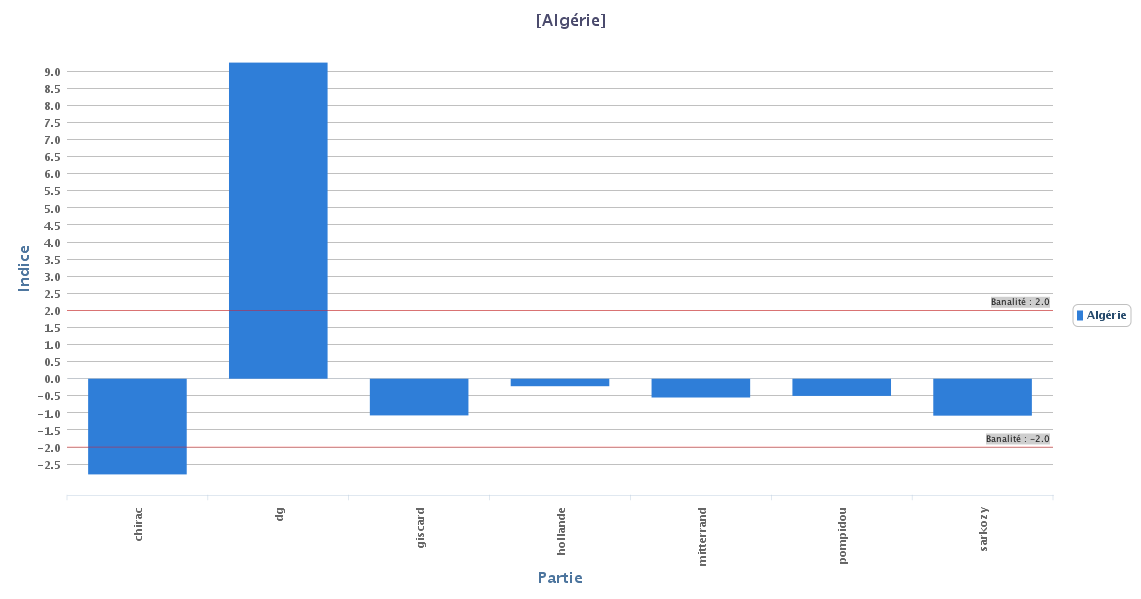
\includegraphics[width=1\linewidth]{img/Algerie.png}
 		\caption{Diagramme en bâtons indiquant les spécificités du mot \texttt{Algérie} dans les discours présidentiels.}
 		\label{fig:specificites_algerie}
 	\end{figure}

\item Nous utilisons deux requêtes : 
\begin{itemize}
	\item \Colorbox{mygray}{\texttt{[frlemma = "États-Unis"\%d]}} (avec la neutralisation des diacritiques)
	\item  \Colorbox{mygray}{\texttt{[frlemma = "Algérie"]}}
\end{itemize}

qui génèrent le graphique de progression cumulative des occurrences des lemmes \texttt{États-Unis} (en rouge) et \texttt{Algérie} (en bleu) sur la Figure \ref{fig:usa_algerie}.
\begin{itemize}
	\item au niveau de la fréquence globale, le lemme \texttt{Algérie} est mentionné deux fois plus souvent, surtout dans les discours associés à de Gaulle (21 occurrences) que \texttt{États-Unis} (11 occurrences) dans l'ensemble du corpus ;
	\item le lemme \texttt{Algérie} est plus fréquemment mentionné et plus tôt dans le corpus (nous observons un saut de courbe, suivi d'un grand plateau), tandis que \texttt{États-Unis} apparaît de manière sporadique et plus tardive (la courbe est moins raide).
\end{itemize}

 	 	\begin{figure}[H] % Use [H] to force the figure to stay in place
 		\centering
 		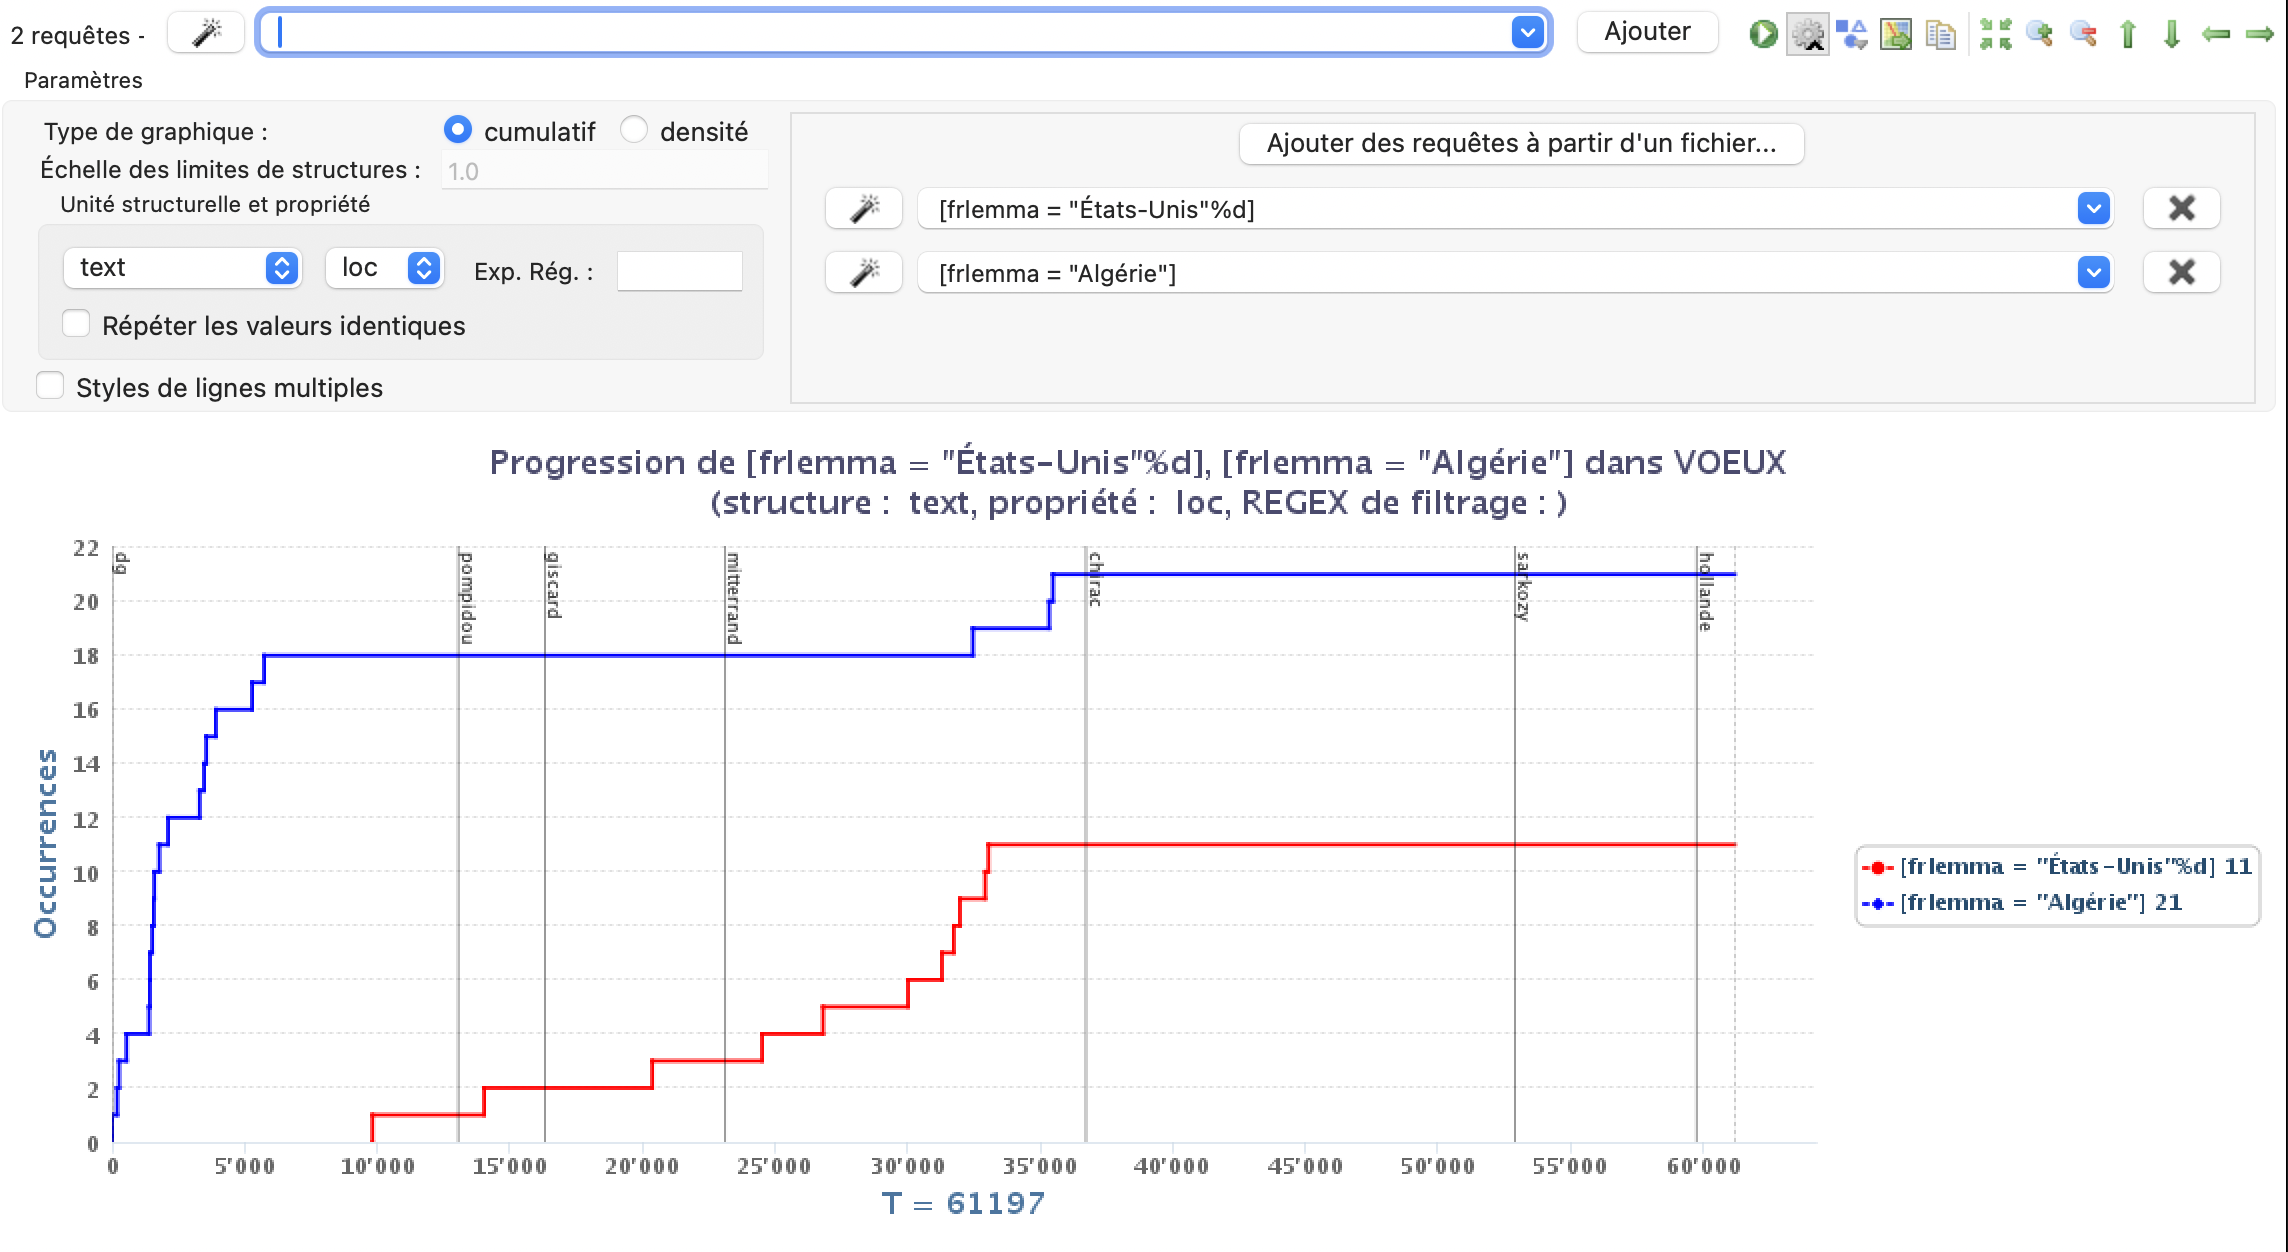
\includegraphics[width=1\linewidth]{img/usa_algerie.png}
 		\caption{Progression des lemmes \texttt{États-Unis} et \texttt{Algérie}.}
 			\label{fig:usa_algerie}
 	\end{figure}
 	
 	\item Hollande, Chirac et Sarkozy sont situés à droite et associés à des mots comme \texttt{chômage}, \texttt{gouvernement}, et \texttt{sécurité}, reflétant des préoccupations modernes et sociales.
 	 	 	\begin{figure}[!h] % Use [H] to force the figure to stay in place
 		\centering
 		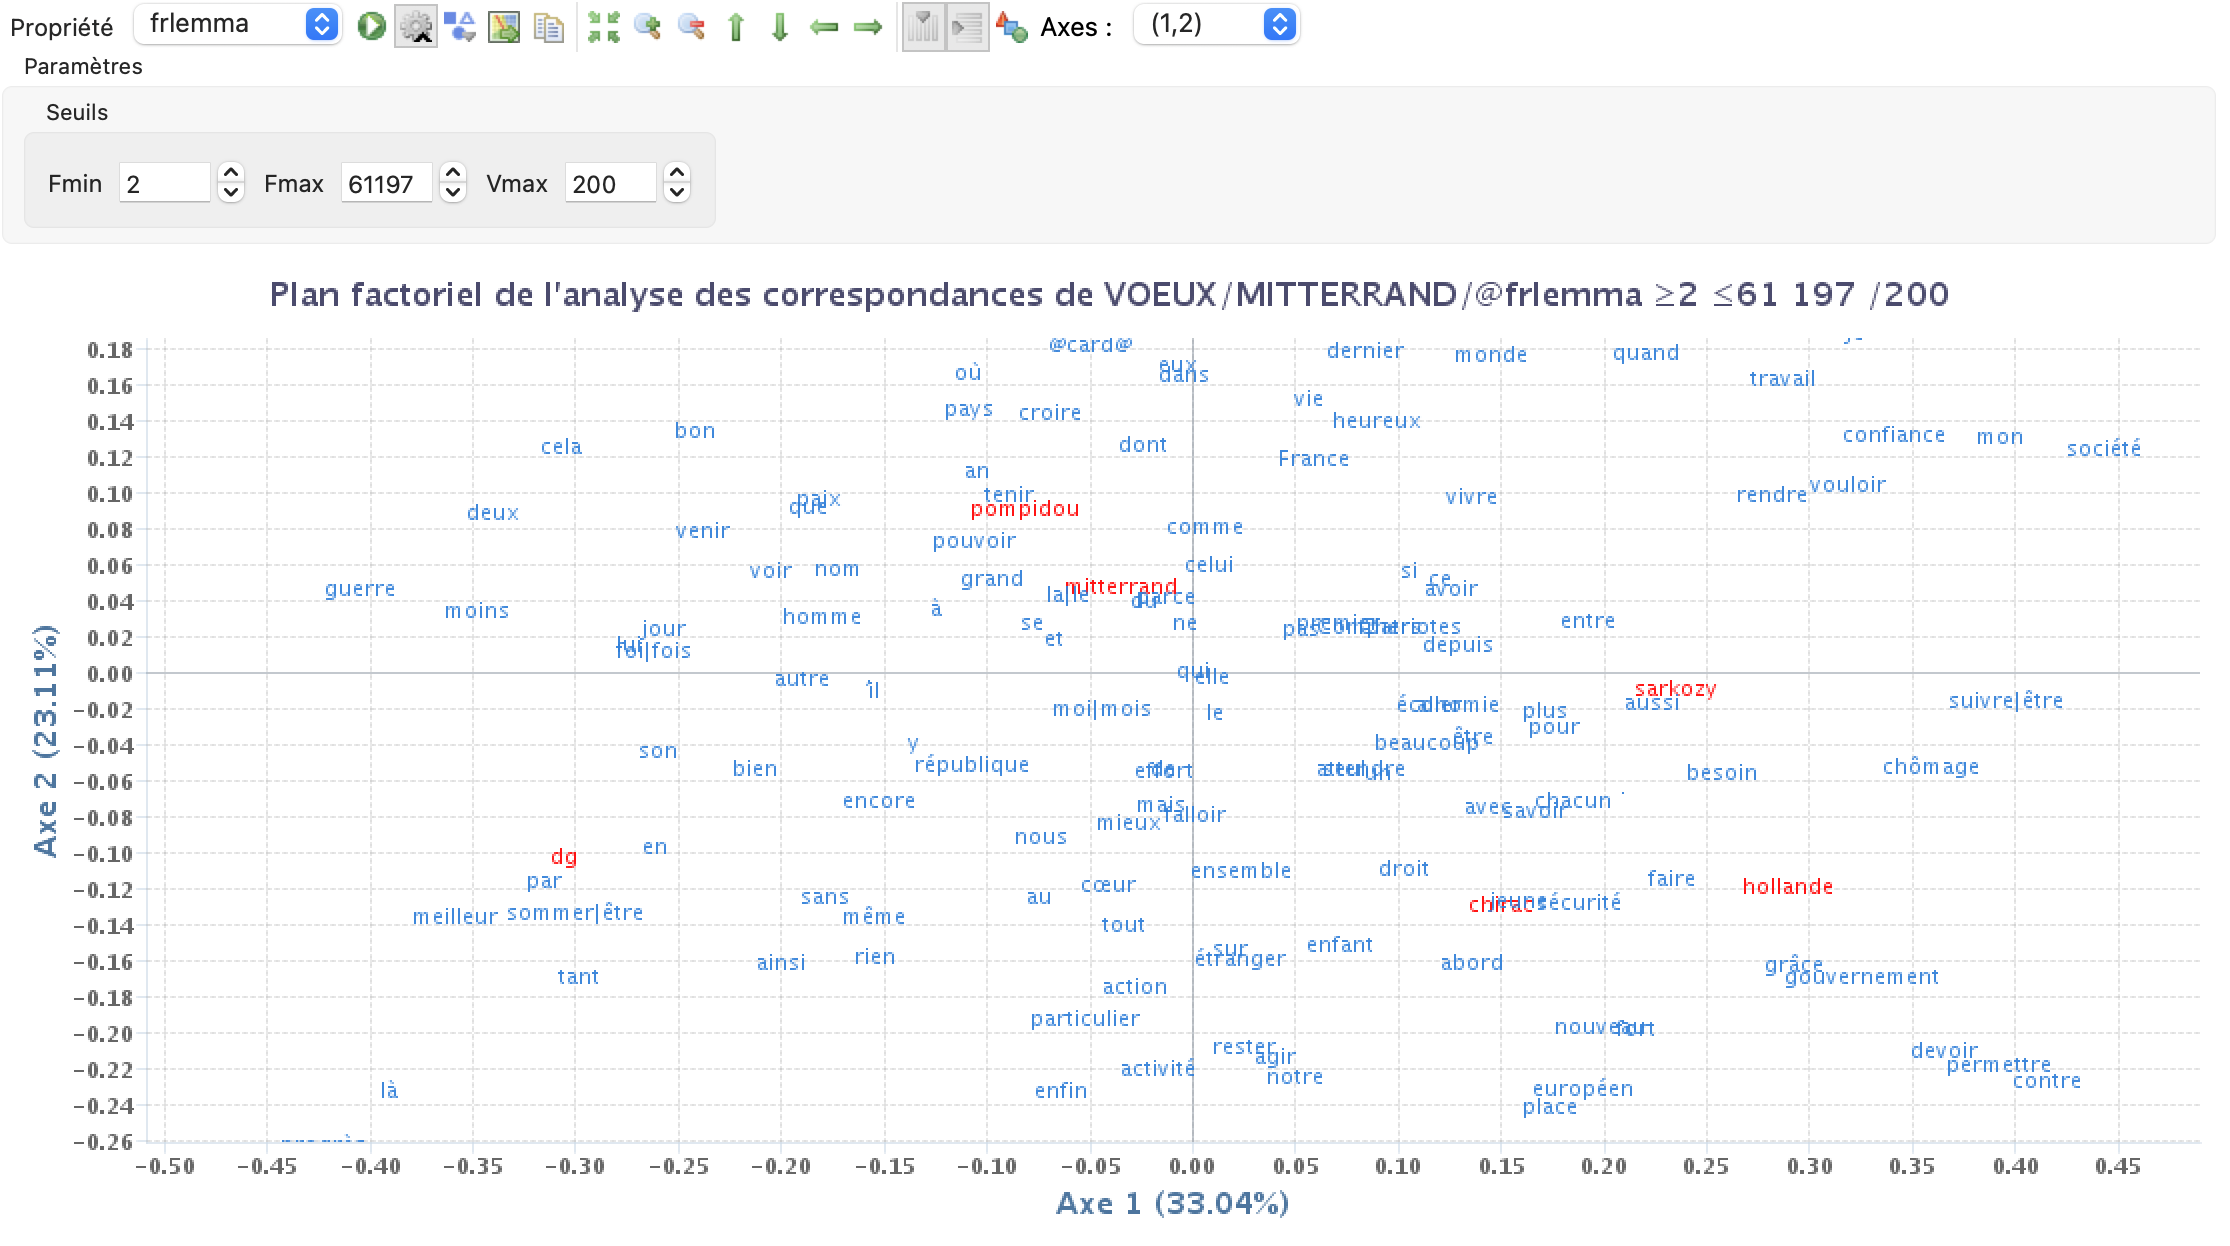
\includegraphics[width=1\linewidth]{img/afc.png}
 		\caption{Analyse factorielle des correspondances -- corpus \texttt{VOEUX}.}
 		\label{fig:usa_algerie}
 	\end{figure}
 	
 	\item Discussion en TD.

\end{enumerate}
 
 	
		\printbibliography



	
\end{document}
